\documentclass[tikz,dvipsnames]{standalone}

\usepackage{amsmath}
\usepackage{amssymb}

\begin{document}

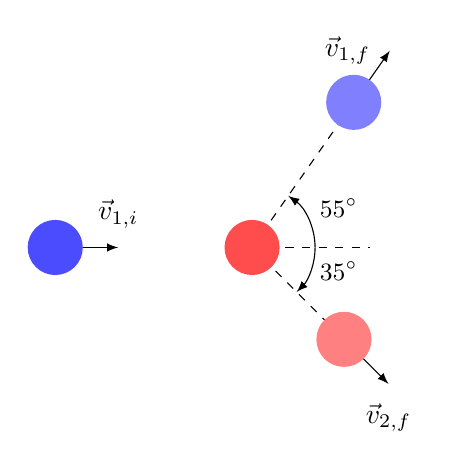
\begin{tikzpicture}
    \fill[blue!70] (-0.5,0) circle (0.35);
    \draw[-latex] (0.35-0.5,0)--(0.8-0.5,0) node [label=above:{$\Vec{v}_{1,i}$}] {};
    \draw[dashed] (2,0)-- (3.5,0);
    \draw[dashed] (2,0) -- ++(55:2.25) node (a){};
    \draw[-latex] (a) -- ++(55:0.8) node [label=left:{$\Vec{v}_{1,f}$}] {};
    \fill[blue!50] (a) circle (0.35);
    \draw[black,-latex] (2.8,0) arc (0:55:0.8) node at (3.1,0.5){\small{$55^\circ$}};
    \draw[dashed] (2,0) -- ++(-45:1.65) node (b){};
    \fill[red!70] (2,0) circle (0.35);
    \draw[black,-latex] (2.8,0) arc (0:-45:0.8) node at (3.1,-0.3){\small{$35^\circ$}};
    \draw[-latex] (b) -- ++(-45:0.8) node [label=below:{$\Vec{v}_{2,f}$}] {};
    \fill[red!50] (b) circle (0.35);
    \end{tikzpicture}

\end{document}

